

\section{Architektur der ApoCo-Datenbank(SQLite)}

Im Buch von Arno Becker und Marcus Pant\cite[S.244]{Android:02}, wird ein Architekturvorschlag f\"ur eine
Datenbankzugriffsschicht f\"ur Android-Anwendungen gemacht.
ApoCo folgt diesem Vorschlag, der hier erl\"autert wird.

\subsection{Motivation}

Beim Umgang mit einer Datenbank ist es oft erw\"unscht eine von der Anwendungsschicht getrennte Zugriffsschicht auf die Datenbank zu haben.
Daf\"ur kann man sich an dem Konzept der Programmierung mit Java-EE orientieren.
Android ist f\"ur ein solches Konzept nicht ausgelegt und so ergeben sich folgende Nachteile:

\begin{itemize}
 
\item Die Anwendung wird ungewollt gro\ss{} und die Performance sinkt.
\item Da keine Frameworks, wie zum Beispiel Spring oder Hibernate existieren, sind \"Anderungen an der Datenbank sehr aufwendig.
\item Es gibt keine M\"oglichkeit die Datenbankschicht von der Pr\"asentationsschicht ohne sp\"urbaren Leistungsabfall zur Laufzeit zu trennen
\cite[S.244]{Android:02}.

\end{itemize}

Au\ss{}erdem wurde festgestellt, dass eine reine Schichtentrennung unm\"oglich ist, 
wenn man mit einem Cursor-Objekt arbeiten m\"ochte.
Der Cursor ist wie ein Zeiger und ist darauf ausgelegt mit gro\ss{}en Datenmengen in einer Datenbank umgehen zu k\"onnen.\\

\subsection{Architekturumsetzung}

Die Zugriffsschicht auf die Android-Datenbank besteht aus den folgenden Klassen:

\begin{itemize}
 \item DBManagerLocal
 \item TabellennameColumns
 \item TabellennameDTO
 \item TabellennameTbl
\end{itemize}

Dabei ist zu beachten, dass f\"ur jede Tabelle eine \emph{Columns, DTO} und \emph{Tbl}-Klasse existiert. 
Die Bezeichnung dieser Klassen setzt sich aus dem Tabellennamen als Pr\"afix und den so eben genannten Klassenendungen zusammen.\\

Die Klasse \emph{DBManagerLocal} ist eine Verwaltungsklasse, um die Datenbank in der Activity greifbar zu machen.
Diese Verwaltungsklasse erweitert die Klasse SQLiteOpenHelper aus dem Android-SDK.
Der SQLiteOpenHelper wei\ss{} wie eine Datenbank erzeugt und ge\"andert wird.
Daf\"ur sind zwei Methoden vorgegeben: \emph{onCreate()} und \emph{onUpgrade()}.
Mit diesen zwei Methoden wird das Datenbankschema aufgebaut und bei \"Anderungen gel\"oscht und neu aufgebaut.
Um einen Backup-Mechanismus muss man sich selbst k\"mmern.
Des Weiteren sind im \emph{DBManagerLocal} Methoden implementiert, um mit der Datenbank Daten auszutauschen.
Im Listing 4.1 wird eine reduzierte Version des \emph{DBManagerLocal} implementiert und es wird eine Tabelle \emph{user} angelegt.
Die Klasse \emph{DBManagerLocal} implementiert die Schnittstelle \emph{DBManagerPreferencesIF}.
In dieser Schnittstelle wird der Name der Datei f\"ur die Datenbank und die Versionsnummer hinterlegt.
Die Versionsnummer ist hier sehr wichtig.
Wird das Datenbankschema ge\"andert, so muss die Versionsnummer inkrementiert werden.
Nur so erkennt die Klasse SQLiteOpenHelper, dass die Datenbank neu aufgebaut werden muss.\\

\begin{lstlisting}[caption={Beispiel f\"ur reduzierte Implementierung der \emph{DBManagerLocal} Klasse}]
 public class DBManagerLocal extends SQLiteOpenHelper implements DBManagerPreferencesIF{ 
 
    public DBManagerLocal(Context context) {
       super(context, DATENBANK_NAME, null, DATENBANK_VERSION);
    } 
    public void onCreate(SQLiteDatabase db) { 
    }    
    public void onUpgrade(SQLiteDatabase db, int oldVersion, int newVersion) {
    }
 }
\end{lstlisting}

Die \emph{TabellennameColumns}-Klassen sind als Schnittstellen und werden pro Tabelle angelegt.
Sie besitzen Konstanten f\"ur jede Spaltenbezeichnung der jeweiligen Tabelle.
Im Listing 4.2 wird ein Beispiel \emph{Columns-Klasse} f\"ur die Tabelle \emph{user} veranschaulicht.\\

\begin{lstlisting}[caption={Die Schnittstelle \emph{UserColumns}}]
 public interface UserColumns {
     static final String _ID      = "_id";
     static final String VORNAME  = "vorname";
     static final String NACHNAME = "nachname";
     static final String EMAIL    = "email";
     static final String PASSWORD = "password";
 }
\end{lstlisting}

Beim Zugriff auf die Tabelle \emph{user} wird im SQL-Statement \"uber die Konstanten der \emph{Columns-Klasse} auf die 
einzelnen Tabellenspalten zugegriffen.
In der Klasse \emph{TabellennameTbl} werden Schemainformationen und SQL-Statements als Konstanten vom Typ String bereitgestellt.
Die Klasse \emph{DBManagerLocal} nutzt die Schemainformationen, um eine Tabelle zu erzeugen.
Die SQL-Statements sind als Prepared Statements zu verstehen.
Das bedeutet, dass sie nur ein SQL-Statement-Muster ohne Parameter repr\"asentieren.
F\"ur Parameter wird das Fragezeichen (\emph{?}) als Platzhalter verwendet, 
das vor dem Zugriff auf die Datenbank durch einen echten Parameter ersetzt wird.
Das Listing 4.3 veranschaulicht mit der \emph{UserTbl} eine Tabellenschema-Klasse.\\

\begin{lstlisting}[caption={Die Klasse \emph{UserTbl}}]
 public final class UserTbl implements UserColumns {
 
    //Tabellenname
    public static final String TABLE_NAME = "user";
    
    //Create-Statement zum Anlegen der Tabelle
    public static final String SQL_CREATE = 
       "CREATE TABLE " + TABLE_NAME + "(" + 
      _ID + " INTEGER PRIMARY KEY AUTOINCREMENT," + 
      VORNAME + " TEXT NOT NULL," + 
      NACHNAME + " TEXT NOT NULL," + 
      EMAIL + " TEXT NOT NULL," + 
      PASSWORD + " TEXT NOT NULL" + ");";
      
   //Drop-Statement zum L\"oschen der Tabelle
   public static final String SQL_DROP = 
      "DROP TABLE IF EXISTS " + TABLE_NAME;
      
   //Beispiel-Statement, welches alle Benutzer mit dem gleichen Nachnamen zurueckgibt.
   //Der Nachname wird als Parameter uebergeben.
   public static final String STMT_GET_USER = 
      "SELECT * FROM " + TABLE_NAME + 
      "WHERE " + NACHNAME + "=?";
}
\end{lstlisting}

Listing 4.4 zeigt ein Beispiel, um die Tabelle \emph{user} zu erzeugen oder sie bei \"Anderungen des Datenbankschemas neu zu erzeugen.
Daf\"ur ruft die \emph{DBManagerLocal}-Klasse die Methode \emph{onCreate()} bzw. \emph{onUpgrade()} automatisch auf.\\

\begin{lstlisting}[caption={\emph{DBManagerLocal} erzeugt die Tabelle \emph{user}}]
 public void onCreate(SQLiteDatabase db) {  
    //erzeuge user-Tabelle
    db.execSQL(UserTbl.SQL_CREATE);
 }
    
 public void onUpgrade(SQLiteDatabase db, int oldVersion, int newVersion) {
    //loesche und erzeuge die user-Tabelle
    db.execSQL(UserTbl.SQL_DROP);
    onCreate(db);
 }
\end{lstlisting}

Beim Aufrufen des DROP- und CREATE-Statements muss wegen der Tabellenabh\"angigkeiten auf die richtige Reihenfolge geachtet werden.
Erstellt werden immer zuerst Tabellen ohne Fremdschl\"ussel und dann der Rest.
Die Tabellen werden in genau umgekehrter Reihenfolge wieder gel\"oscht.
Die \emph{TabellennameDTO}-Klassen sind einfache Container-Klassen und erm\"oglichen einen objektorientierten Umgang mit den Ergebnissen aus Datenbankanfragen oder 
das \"Ubergeben eines \emph{DTO}-Objekts an die Datenbank zum Speichern.
Im Listing 4.5 wird eine stark reduzierte \emph{DTO}-Klasse f\"ur die Tabelle \emph{user} veranschaulicht.
Die \emph{DTO}-Klassen haben Felder, die den Spalten der Tabelle entsprechen, welcher sie angeh\"oren.
Ein \emph{DTO}-Objekt kann auf verschiedene Arten entstehen.
Aus Parametern, die sich aus Messungen und Benutzereingaben ergeben, 
aus einer Datenbankanfrage, die einen Cursor liefert oder einem JSON-Objekt aus einer Anfrage an den Webserver.
Es kann auch notwendig sein ein Objekt mit einem Standardkonstruktor zu erzeugen und die Felder sp\"ater zu initialisieren.
F\"ur diese F\"alle werden vier Konstruktoren ben\"otigt.
Nicht jede \emph{DTO}-Klasse ben\"otigt immer alle vier Konstruktoren.\\

\begin{lstlisting}[caption={\emph{UserDTO}-Klasse in leicht reduzierter Form}]
public class UserDTO {

   public long _id;
   public String vorname;
   public String nachname;
   public String email;
   public String password;
   
   
   public UserDTO(){};
   public UserDTO(long, String, String, Sting, String){...}
   public UserDTO(Cursor){...}
   public UserDTO(JSONObject){...}
   //getter & setter
   
   public JSONObject toJSONObject() {... return jsonObj;}
}
\end{lstlisting}

Eine wichtige Methode jeder \emph{DTO}-Klasse ist die \emph{toJSONObject()}-Methode.
F\"ur den Fall, dass Messungen oder Benutzereingaben an den Webserver geschickt werden m\"ussen,
geschieht dies \"uber eine REST-Schnittstelle mit einem JSON-String.
Um es so einfach wie m\"oglich zu halten die Objekte als Parameter an die REST-Schnittstelle zu senden,
hat jedes Objekt die F\"ahigkeit seine gespeicherten Eigenschaften als ein JSON-Objekt zur\"uckzugeben.
Die Implementierung dieser Methode veranschaulicht das Listing 4.6.\\

\begin{lstlisting}[caption={\emph{UserDTO}-Klasse in leicht reduzierter Form}]
public class UserDTO {
   public JSONObject toJSONObject() {
      JSONObject obj = new JSONObject();
      try {
         obj.put(UserTbl._ID, this._id);
         obj.put(UserTbl.VORNAME, this.vorname);
         obj.put(UserTbl.NACHNAME, this.nachname);
         obj.put(UserTbl.EMAIL, this.email);
         obj.put(UserTbl.PASSWORD, this.password);
      } catch (JSONException e) {
         Log.d(CLAZZ_NAME, "toJSONObject failed: " + e.getMessage());
      }
      return obj;
   }
}
\end{lstlisting}
Das Listing 4.6 demonstriert auch gleichzeitig wie die \emph{Tbl}-, \emph{Columns}- und \emph{DTO}-Klassen zusammenarbeiten.
Um die richtige Spaltenbezeichnung zu nutzen, greift die \emph{DTO}-Klasse \"uber die \emph{Tbl}-Klasse auf die \emph{Columns}-Schnittstelle 
und dort auf die Konstanten der Spaltennamen zu.
Damit eine Activity mit dem \emph{DBManagerLocal} auf die Datenbank Zugriff bekommt, 
m\"ussen Methoden f\"ur den Zugriff in der Klasse \emph{DBManagerLocal} implementiert werden.
Im Listing 4.3 wird bereits das SQL-Statement \emph{\texttt{STMT\_GET\_USER}} in der \emph{UserTbl}-Klasse gezeigt.
Dieses Statement nutzt der \emph{DBManagerLocal} in einer eigenen Methode, um eine Anfrage daraus zu bauen.
Eine Beispielanfrage wird mit dem Listing 4.7 demonstriert.\\

\begin{lstlisting}[caption={Methode \emph{getUserByNachname()} der \emph{DBManagerLocal}-Klasse}]
public class DBManagerLocal ... {
   ...
   //Methode fuer eine Datenbankanfrage
   public Cursor getUserByNachname(UserDTO user) throws SQLException{
      //Hier wird der Nachname aus dem DTO-Objekt als Parameter in einem String-Array gespeichert.
      String[] param = {user.nachname};
      //getReadableDatabase liefert eine Referenz auf ein Objekt, welches die Datenbankverbindung zum Lesen oeffnet.
      //das Statement aus der Klasse UserTbl und die Parameter werden an die Methode rawQuery uebergeben.
      //rawQuery liefert einen Cursor auf die Antwort aus der Datenbank.
      Cursor cursor = getReadableDatabase().rawQuery(UserTbl.STMT_GET_USER, param);
      return cursor;
   }   
}
\end{lstlisting}

Das Ergebnis der Anfrage kann in einer Activity anschlie\ss{}end ausgewertet werden.
Eine Demonstration liefert das Listing 4.8.
Hier wird zuerst mit dem if-Statement gepr\"uft, ob ein Ergebnis in der Datenbank gefunden wurde.
Die while-Schleife bewegt beim ersten Durchlauf den Cursor auf die erste Zeile der Antwort.
Im Rumpf der while-Schleife werden die Ergebnisse bearbeitet, und das so lange bis die Methode moveToNext() ein false liefert.\\

\begin{lstlisting}[caption={Methode \emph{getUserByNachname()} der \emph{DBManagerLocal}-Klasse}]
public class MyActivity... {
   ...    
   DBManagerLocal dbManager = new DBManagerLocal(MyActivity.this);      
   
   public void todo() {         
      Cursor result = dbManager.getUserByNachname(user);      
      if (result.getCount() > 1) {      
         while(result.moveToNext()) {         
            UserDTO user = new UserDTI(result); ...
         }
      }
   }
}
\end{lstlisting}

\subsection{ApoCo Datenbankdiagramm}

In der Abbildung 4.4 wird das ApoCo Datenbankschema als Klassendiagramm dargestellt.
Die Abk\"urzungen \emph{FK1, FK2} stehen dabei f\"ur Fremdschl\"ussel. Die Prim\"arschl\"ussel werden als Schl\"usselsymbol dargestellt.
Folgende Tabellen sind im Diagramm zu sehen:

\begin{itemize}
 \item user:\\
 Diese Tabelle enth\"alt Daten der Patienten.
 Die ApoCo-Anwendung ist so konzipiert, dass sie mehrere Patienten auf einem Smartphone verwalten kann.
 Jeder Patient hat seine eigenen Anmeldedaten und kann die Daten der anderen Patienten nicht einsehen.
 
 \item bloodpressure:\\
 In dieser Tabelle werden Messprotokolle f\"ur den Blutdruck persistent gespeichert.
 Neben dem Datum und den Spalten f\"ur die Messwerte ist hier noch eine weitere Spalte mit der Bezeichnung \emph{sync} zu sehen.
 Diese Spalte ist f\"ur die Synchronisation der Daten mit dem Webserver norwendig.
 Es handelt sich dabei um einen Flag der von 0 auf 1 gesetzt wird, wenn die Messwerte an den Webserver \"ubertragen wurden.
 
 \item bodyweight:\\
 Die Tabelle \emph{bodyweight} speichert Messdaten zum K\"orpergewicht.
 Auch hier ist ebenfalls eine Flag-Spalte f\"ur den Synchronisationsvorgang.
 
 \item mealenergy:\\
 Die Tabelle \emph{mealenergy} repr\"asentiert pro Eintrag eine ganze Mahlzeit.
 Hier wird nur festgehalten wann die Mahlzeit eingenommen wurde und ob die Mahlzeit mit dem Webserver synchronisiert ist.
 
 \item \texttt{mealenergy\_content}:\\
 Diese Tabelle enth\"alt einzelne Positionen einer Mahlzeit.
 Sie speichert aber nur das Gewicht und die Energiemenge der jeweiligen Position, wie auch die dazugeh\"orige EAN-Nummer.
 Die Tabellen \emph{mealenery} und \emph{\texttt{mealenergy\_content}} bilden somit eine Einheit bei der Berechnung von Energieaufnahme 
 durch die Nahrung.
 
 \item food:\\
 Die Tabelle \emph{food} dient als Erg\"anzung der Positionen einer Mahlzeit.
 Jedes Lebensmittel, das zum ersten Mal mit Hilfe des Barcodescanners erkannt wurde, wird hier f\"ur schnellen Zugriff gespeichert.
 
 \item tageseinheiten:\\
 Der Arzt gibt seinen Patienten vor, wieviel Kilokalorien sie am Tag zu sich nehmen d\"urfen.
 Die aktuellen Werte werden vom Webserver geladen und in dieser Tabelle abgelegt.
\end{itemize}

\begin{figure}[h]
  \centering
  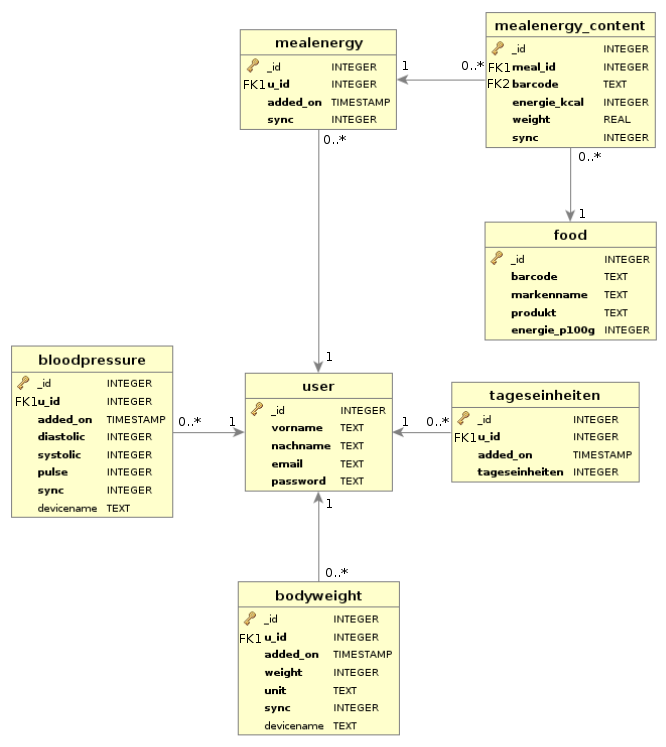
\includegraphics[scale=0.53]{diagramme/kapitel4/apoco_datenbank_schema.png}
  \caption{ApoCo Datenbankdiagramm}
  
\end{figure}
